\chapter{Complex event processing}
	\label{chap:cep}
	\section{Intro of the Complex Event Processing}
		In this hierarchical runtime verification project, the top level of modelling is done in an event pattern language.
		This event pattern language is translated to timed event automatons. These event automatons will be executed in the
		process.
	\section{Formal Intro of the Timed Parametrized Event Automaton}
		\subsection{VEPL}
			Our choice for the event pattern definition is the VIATRA Event Pattern Language (VEPL).
			Currently this is the only CEP which can be easily integrated to a live model, where 
			you can define multiple patterns over the model, and define atomic events for the (dis)appereance
			of these patterns.
			
			TODO define complex event processing
			
			A brief overview of the VEPL language:

\begin{tabular}{ccc}
\centering
Operator name &	Denotation & Meaning \\
followed by & p1 $\rightarrow$ p2 & Both patterns have to appear in the specified order. \\
or &	p1 OR p2 &	One of the patterns has to appear. \\
and &	p1 AND p2 &	Both of the patterns has to appear, but the order does not matter. Rule: p1 AND p2 === ((p1 $\rightarrow$ p2) OR (p2 $\rightarrow$ p1)). \\
negation &	NOT p &	On atomic pattern: event instance with the given type must not occur. On complex pattern: the pattern must not match. \\
multiplicity &	p\{n\} &	The pattern has to appear n times, where n is a positive integer. Rule: p\{n\} === p1 $\rightarrow$ p1 $\rightarrow$ ... p1, n times. \\
"at least once" multiplicity &	p\{+\} &	The pattern has to appear at least once. \\
"infinite" multiplicity &	p\{*\} &	The pattern can appear 0 to infinite times. \\
within timewindow &	p[t] &	Once the first element of the pattern is observed (i.e. the patterns "starts to build up"), the rest of the pattern has to be observed within t milliseconds.
\end{tabular}	
			
			%% Regular -> Timed Regular -> Event Automata (parametrized) -> MERGE -> Timed Event Automaton
		\subsection{Timed Regular Expression}
			\begin{dfn}
				Timed Regular Expressions over an alphabet $\Sigma$ (also referred to as $\Sigma$-expressions)
				are defined using the following families of rules.
				\begin{enumerate}
					\item{\underline{a} for every letter $a \in \Sigma$ and the special symbol $\varepsilon$ are expressions}
					\item{If $\varphi, \varphi_1, \varphi_2$ are $\Sigma$-expressions and $I$ is an integer-bounded interval then
						$\langle\varphi_I\rangle, \varphi_1~\cdot~\varphi_2, \varphi_1 \vee \varphi_2,$ and $\varphi^\ast$ are $\Sigma$-expressions}
					\item{If $\varphi, \varphi_1$ and $\varphi_2$ are $\Sigma$-expressions then $\varphi_1 \circ \varphi_2, \varphi^\circledast$ are
						$\Sigma$-expressions}
					\item{If $\varphi_1$ and $\varphi_2$ are $\Sigma$-expressions, $\varphi_0$ is a $\Sigma_0$-expression
						for some alphabet $\Sigma_0$, and $\Theta$ : $\Sigma_0 \rightarrow \Sigma$ is
						a renaming, then $\varphi_1 \wedge \varphi_2$ and $\Theta(\varphi_0)$ are $\Sigma$-expressions}
				\end{enumerate}
			\end{dfn}
			
		
		\subsection{Event Automaton}
			% informal definition
			An Event Automaton is a non-deterministic finite-state automaton whose alphabet consists
			of parametric events and whose transitions may be labelled with guards and assignments
			
			% formal definition
			\begin{dfn}
				An EA
				$\langle Q,\mathcal{A},\delta, q_0, F \rangle$ is a tuple where Q is a finite set of states, 
				$\mathcal{A} \subseteq Event$ is a finite alphabet,
				$\delta \in (Q \times \mathcal{A} \times Guard \times Assign \times Q)$ is a finite set of transitions, 
				$q_0 \in Q$ is an initial state, and 
				$F \subseteq Q$ is a set of final states.
			\end{dfn}
			
		\subsection{Timed Event Automaton}
			% stuff about the calendar
			% informal definition of the calendar?
			% In discrete event simulation, a calendar (also called event list) is a data structure that
			% stores future events and the times at which these events are scheduled to occur
			
			% Formal definition of the calendar
				% \begin{dfn}
				% A calendar is a finite set (or multiset) of the form $C = \{ \langle e_1, t_1\rangle \, \dots ,\langle e_n, t_n\rangle \}$
				% where each $e_i$ is an event and $t_i$ is the time when event $e_i$ is scheduled to occur. All $t_i$s are real numbers.
				% We denote by min(C) the smallest number among $\{t_1,\dots ,t_n \}$ (with min(C) = $+\infty$ if C is empty)
				% Given a real u, we denote by $Ev_u(C)$ the subset of C that contains all events scheduled at time u:
				% $Ev_u(C) = \{ \langle e_i, t_i \rangle  | t_i = u \wedge \langle e_i , t_i \rangle \in C \} $
				% \end{dfn}
			% stuff about the calender automaton
				
			\begin{dfn}
				A TimedZone $\langle S,\mathcal{E},I,T \rangle $ is a tuple where $S \in$ States,
				$T \in$ States, 
				$\mathcal{E}~\subseteq$~States,
				$I$ is a time value 
			\end{dfn}
			
			The semantic of the TimedZone is the following: 
				If a token enters state $S$ at $t_i$, and doesn't reach any of the $\mathcal{E}$ states before $t_j$,
				where $t_j = t_i + I$, then the token is moved to $T$
				
			\begin{dfn}
				A TEA
				$\langle E,\mathcal{T} \rangle$ is a tuple where $E$ is an Event Automaton, and $\mathcal{T}$ is a set of Timed Zones, where all the states are one of the 
				Automatons states.
			\end{dfn}

	\section{Examples of Event Processing}
 
		\subsection{File System}
			\subsubsection{Problem}
				File system - A file shouldn't be read when it has been opened for writing, and shouldn't be written, when opened for reading. 
				A file shouldn't be opened for writing and reading without a close event between the two different opens.
				The possible parametrized events are : 
				Open(file, mode), 
				Close(file), 
				Read(file), 
				Write(file). 
				Mode is either "R" or "W" which stands for Read and Write respectively.
			\subsubsection{Solution}
				We are looking for these patterns : 
				
				open(f,"W") $\rightarrow$ NOT close(f)$\{\ast\}$ $\rightarrow$ open(f,"R");
				
				open(f,"R") $\rightarrow$ NOT close(f)$\{\ast\}$ $\rightarrow$ open(f,"W");
				
				open(f,"W") $\rightarrow$ NOT close(f)$\{\ast\}$ $\rightarrow$ read(f);
				
				open(f,"R") $\rightarrow$ NOT close(f)$\{\ast\}$ $\rightarrow$ write(f);
				
				\begin{figure}[h]
				\centering
				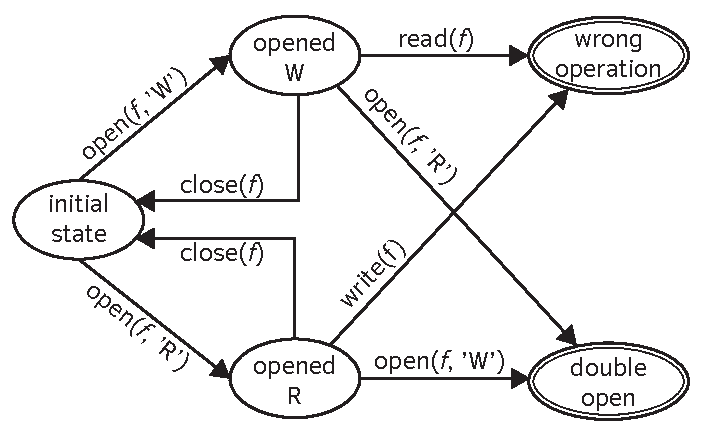
\includegraphics[width=0.7\linewidth]{include/figures/chapter_5/file_example_aut}
				\caption{Automaton of the file example}
				\label{fig:cep:fileautomaton}
				\end{figure}

		
		
		\subsection{Mars Rover Tasking - Two phase locking}
			\subsubsection{Problem}
				In concurrent systems the avoidance of deadlocks and livelocks are an utmost importance.
				To solve this problem, one of the many patterns is  the two phase locking - which can be defined by two rules.
				These rules are : 
				\begin{enumerate}
					\item{Every task must allocate the resources in a given order.}
					\item{If a task releases a resource, it can't allocate anymore}
				\end{enumerate}
			\subsubsection{Solution}
				Since our implementation doesn't support guards \emph{yet} we can only use constant amount of resources.
				For this example, this amount will be set to two, to minimise the model of the example.

				\begin{figure}[h]
				\centering
				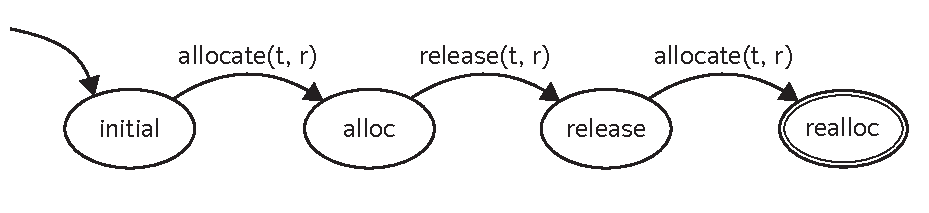
\includegraphics[width=0.7\linewidth]{include/figures/chapter_5/mars_example_aut1}
				\caption{Automaton to forbid the reallocation}
				\label{fig:cep:marsautomaton1}
				\end{figure}		
				
				
				\begin{figure}[h]
				\centering
				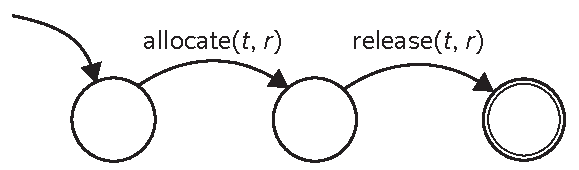
\includegraphics[width=0.7\linewidth]{include/figures/chapter_5/mars_example_aut2}
				\caption{Automaton to forbid inverse allocation}
				\label{fig:cep:marsautomaton2}
				\end{figure}	

				
				
	\section{Implementation}
		\subsection{Metamodel}
		
			\begin{figure}[h]
			\centering
			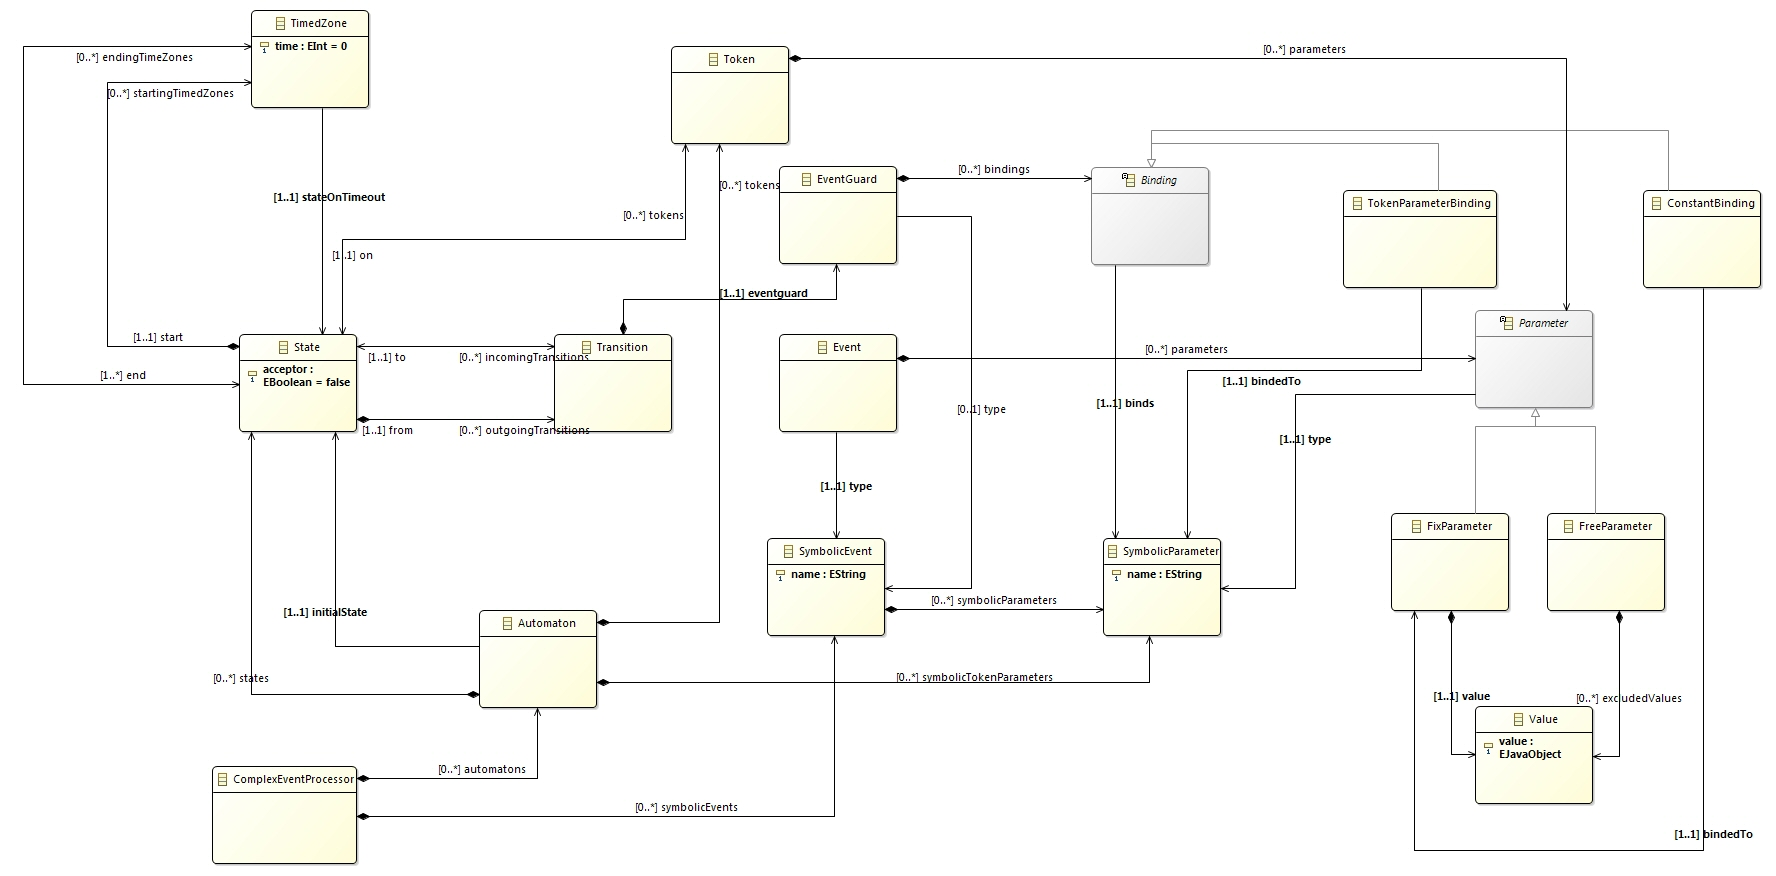
\includegraphics[width=0.9\linewidth]{include/figures/chapter_5/model}
			\caption{Automaton of the file example}
			\label{fig:cep:model}
			\end{figure}
		%image
		Nyilvan ide majd kisebb, mutatosabb, es kevesebb dolgot tartalmazo abra kell, meg nemi magyarazat
		Egy csak timedZones resz, meg egy csak parameteres
		\subsection{Executor}
			The algorithm first searches for all the activated transitions.
			If it finds an activated transition, it iterates over the tokens which are on the state. The first token with matching (non-confronting)
			parameter list will be split to the next state if there are new parameter bindings from the event, or moved if there are no new bindings.
			If a token enters an acceptor state it'll 
			next state 
